\documentclass[10pt]{article}

\usepackage{amsmath,amscd}
\usepackage{amssymb,array}
\usepackage{amsfonts,latexsym}
\usepackage{graphicx,subfig,wrapfig}
\usepackage{times}
\usepackage{psfrag,epsfig}
\usepackage{verbatim}
\usepackage{tabularx}
\usepackage[pagebackref=true,breaklinks=true,letterpaper=true,colorlinks,bookmarks=false]{hyperref}
\usepackage{ mathrsfs }

\DeclareMathOperator*{\rank}{rank}
\DeclareMathOperator*{\trace}{trace}
\DeclareMathOperator*{\range}{range}
\DeclareMathOperator*{\spn}{span}
\DeclareMathOperator*{\acos}{acos}
\DeclareMathOperator*{\argmax}{argmax}

\newcommand{\matlab}[1]{\texttt{#1}}
\newcommand{\setname}[1]{\textsl{#1}}
\newcommand{\Ce}{\mathbb{C}}

\newenvironment{mfunction}[1]{
\noindent
\tabularx{\linewidth}{>{\ttfamily}rX}
\hline
\multicolumn{2}{l}{\textbf{Function \matlab{#1}}}\\
\hline
}{\\\endtabularx}

\newcommand{\parameters}{\multicolumn{2}{l}{\textbf{Parameters}}\\}

\newcommand{\fdescription}[1]{\multicolumn{2}{p{0.96\linewidth}}{

\textbf{Description}

 #1}\\\hline}

\newcommand{\retvalues}{\multicolumn{2}{l}{\textbf{Returned values}}\\}
\def\0{\boldsymbol{0}}
\def\b{\boldsymbol{b}}
\def\bmu{\boldsymbol{\mu}}
\def\e{\boldsymbol{e}}
\def\u{\boldsymbol{u}}
\def\x{\boldsymbol{x}}
\def\v{\boldsymbol{v}}
\def\w{\boldsymbol{w}}
\def\N{\boldsymbol{N}}
\def\X{\boldsymbol{X}}
\def\Y{\boldsymbol{Y}}
\def\A{\boldsymbol{A}}
\def\B{\boldsymbol{B}}
\def\y{\boldsymbol{y}}
\def\cX{\mathcal{X}}
\def\transpose{\top} 

%\long\def\answer#1{{\bf ANSWER:} #1}
\long\def\answer#1{}
\newcommand{\myhat}{\widehat}
\long\def\comment#1{}
\newcommand{\eg}{{e.g.,~}}
\newcommand{\ea}{{et al.~}}
\newcommand{\ie}{{i.e.,~}}

\newcommand{\db}{{\boldsymbol{d}}}
\renewcommand{\Re}{{\mathbb{R}}}
\newcommand{\Pe}{{\mathbb{P}}}

\hyphenation{MATLAB}
\usepackage[margin=1in]{geometry}


\begin{document}

\title{
\vspace{-19mm}
Computer Vision (600.461/600.661)\\
Homework 5: Two View Geometry and Optical Flow}
\author{Greg Kiar}


\maketitle

\begin{enumerate}

\item \textbf{(20 points) Properties of $so(3)$ and $SO(3)$.}
\begin{enumerate}

%q1a
\item Given the structure of $\hat{w}$, we can determine its rank and nullspace as follows
\begin{align*} \hat{w} &= \begin{bmatrix} 0 & -w_3 & w_2 \\ w_3 & 0 & -w_1 \\ -w_2 & w_1 & 0 \end{bmatrix} \\
\end{align*}
When we apply the following linear operation on $w_3$, we see that the rows are linearly dependent on one another. $\therefore rank(\hat{w}) = 2$.
\begin{align*} w_3 = w_1 \frac{-w_1}{w_3} + \frac{-w_2}{w_3} \end{align*}
By definition, $\hat{w} = w \times A$, where $A$ is a arbitrary vector. $\therefore \hat{w} w = 0$. We can conclude from this that $w$ is the nullspace of $\hat{w}$, since $w$ is parallel to $\hat{w}$.

%q1b
\item We can solve for $\hat{w}^2$ is shown below
\begin{align*} \hat{w} &= \begin{bmatrix} 0 & -w_3 & w_2 \\ w_3 & 0 & -w_1 \\ -w_2 & w_1 & 0 \end{bmatrix} \\
\hat{w}^2 &=  \begin{bmatrix} 0 & -w_3 & w_2 \\ w_3 & 0 & -w_1 \\ -w_2 & w_1 & 0 \end{bmatrix} \times  \begin{bmatrix} 0 & -w_3 & w_2 \\ w_3 & 0 & -w_1 \\ -w_2 & w_1 & 0 \end{bmatrix} \\
&=  \begin{bmatrix} -w_2^2-w_3^2 & w_1w_2 & w_1w_3 \\ w_1w_2 & -w_1^2-w_3^2 & w_2w_3 \\ w_1w_3 & w_2w_2 & -w_1^2-w_2^2 \end{bmatrix} \\
&= \begin{bmatrix} w_1^2 & w_1w_2 & w_1w_3 \\ w_1w_2 & w_2^2 & w_2w_3 \\ w_1w_3 & w_2w_2 & w_3^2 \end{bmatrix} - \begin{bmatrix} w_1^2 +w_2^2 + w_3^2 & 0 & 0 \\ 0 & w_1^2 + w_2^2 +w_3^2 & 0 \\ 0 & 0 & w_1^2 + w_2^2+w_3^2 \end{bmatrix} \\
\hat{w}^2 &= ww^T - \lVert w \rVert^2 I
\end{align*}
Now, similarly for $\hat{w}^3$
\begin{align*}
\hat{w}^3 &= \hat{w} \hat{w}^2 \\
&= \hat{w} (ww^T - \lVert w \rVert^2 I) \\
&= \hat{w}ww^T - \hat{w} \lVert w \rVert ^2 \\
\hat{w}^3 &= \lVert w \rVert^2 \hat{w}
\end{align*}

%q1c
\item $R$ is found by solving the following differential equation as a discrete time system
\begin{align*}
R(t)R(t)^T &= I \\
\dot{(R(t)R(t)^T)}&= \dot{I} \\
\dot{R}(t)R(t)^T + R(t)\dot{R(t)}^T &= 0 \\
\dot{R}(t)R(t)^T &= -R(t)\dot{R}(t)^T \\
\dot{R}(t)R(t)^T &= - (\dot{R}(t)R(t)^T)^T \\
\hat{w} &= \dot{R}(t)R(t)^T \\ \text{Now,}\\
\dot{R}(t)R(t)^TR(t) &= \hat{w}R(t) \\
\dot{R}(t) &= \hat{w}R(t) \\
\end{align*}
Where $\hat{w}$ is now set to be skew symmetric matrix $R(t)'R^T$ is, solving this using the laplace transform yeilds the following
\begin{align*}
\dot{R}(t) &= \hat{w}R(t) \\
\mathscr{L}\begin{Bmatrix} \dot{R}(t) \end{Bmatrix} &= \mathscr{L} \begin{Bmatrix} \hat{w}R(t) \end{Bmatrix} \\
sR(s) - R_0 &= \hat{w}R(s) \\
R(s) &= \frac{R_0}{\hat{w} + s} \\
\mathscr{L}^{-1} \begin{Bmatrix}R(s) \end{Bmatrix} &= \mathscr{L}^{-1} \begin{Bmatrix} \frac{R_0}{\hat{w} + 1} \end{Bmatrix} \\
R(t) &= R_0 exp(\hat{w}t)
\end{align*}

%q1d
\item A simplification of $R$ from the result obtained above is as follows
\begin {align*} R &= exp(\hat{w} \theta) \\
&= \sum_{n=0}^{\infty} \frac{(\hat{w}\theta)^n}{n!} \\
&= \sum_{n=0}^{\infty} \frac{\hat{w}^n}{n!} \sum_{n=0}^{\infty} \frac{\theta^n}{n!} \\
\end{align*}
We know from expanding the properties of $\hat{w}$ discovered above, that $\hat{w} = - \hat{w}^3$, $\hat{w} = \hat{w}^4$. We also know that $\hat{w}^2 = - \hat{w}^4$, $\hat{w} = \hat{w}^6$. From this we can state the following
\begin{align*} R &= \hat{w}^0 + \hat{w} \sum_{n=0}^{\infty} \frac{(-1)^{n}(\theta)^n}{n!} + \hat{w}^2 \sum_{n=0}^{\infty} \frac{(-1)^{n+1}\theta^n}{n!} \\
&= I+ \hat{w} \sum_{n=0}^{\infty} \frac{(-1)^{n}(\theta)^n}{n!} + \hat{w}^2 \sum_{n=0}^{\infty} \frac{(-1)^{n+1}\theta^n}{n!}
\end{align*}
Applying infinite series expansion we find that
\begin{align*}
R &= I + \sin(\theta)\hat{w} + (1-cos(\theta))\hat{w}^2
\end{align*}
%q1e 
\item The trace of R is computed as follows
\begin{align*} tr(R) &= tr(I + \sin(\theta) \hat{w} + (1 - \cos(\theta))\hat{w}^2) \\
&= tr(I) + tr(\sin(\theta) \hat{w}) + tr((1 - \cos(\theta))\hat{w}^2)\\
&= 3 + tr \begin{pmatrix} \sin(\theta) \begin{bmatrix}0&-w_3&w_2\\w_3&0&-w_1\\-w_2&w_1&0\end{bmatrix} \end{pmatrix} + tr((1-\cos(\theta))(ww^T - \lVert w \rVert^2I)) \\
&= 3 + (1 - cos(\theta)) tr \begin{pmatrix} \begin{bmatrix}w_1^2 & w_1w_2 & w_1w_3 \\ w_1w_2 & w_2^2 & w_2w_3 \\ w_1w_3 & w_2w_2 & w_3^2 \end{bmatrix} - \begin{bmatrix}1&0&0\\0&1&0\\0&0&1 \end{bmatrix} \end{pmatrix} \\
&= 3 + (1 - cos(\theta)) (1 - 3)\\
&= 3 - 2(1 - cos(\theta)) \\
tr(R) &= 1 + 2 cos(\theta)
\end{align*}

%q1f
\item We show that $\w$ is an eigen vector of $R$ below.
\begin{align*}
R \w &= \begin{pmatrix}I - \sin(\theta) \hat{w} + (1-cos(\theta)\hat{w}^2 \end{pmatrix} \w \\
R \w &= I \w \\
R \w & = \w \\
\end{align*}
We can see that $\w$ is an eigen vector for $R$ for the eigen value of $\lambda = 1$.

\end{enumerate}

\item \textbf{(15 points) Optical flow of a perspective camera.}
\begin{enumerate}

%q2a
\item The optical flow of a perspective projection at $t=0$ can be given using the following calculation
\begin{align*}
\x(t) &= \pi \begin{pmatrix}R(t)\X + T(t) \end{pmatrix} \\
&= R(t) \frac{\X}{Z} + T(t) \frac{1}{Z} \\
\dot{\x} &= \dot{R}(t) \x + \dot{T}(t) \frac{1}{Z} \\
\end{align*}
Where $\dot{R}(t)R(t)^T = \hat{w}(t)$, and $ \because R(0)=I$, $\dot{R}(t) = \hat{w}$. For clarity let $w(t) = \w$.
\begin{align*}
\dot{\x} &= \hat{\w}\x + \frac{1}{Z}\v\\
&= -\hat{\x}\w + \frac{1}{Z}\v\\
(I-\x e_3^T)\dot{\x} &= -(I-\x e_3^T)\hat{\x}\w + \frac{1}{Z}(I-\x e_3^T)\v\\
\begin{bmatrix} \dot{\x} \\ \dot{y} \\ 0 \end{bmatrix} &= (-\hat{\x} + \x e_3^T\hat{\x})\w + \frac{1}{Z}(I - \x e_3^T)\v \\
\begin{bmatrix} \dot{x} \\ \dot{y}  \\ 0 \end{bmatrix} &= \begin{pmatrix} -\begin{bmatrix}0&-1&y\\1&0&-x\\-y&x&0 \end{bmatrix} + \begin{bmatrix}-xy&-x^2&0\\-y^2&xy&0\\y&x&0\end{bmatrix} \end{pmatrix} \w + \frac{1}{Z} \begin{bmatrix} 1 & 0 & -x \\ 0& 1 & -y \\ 0&0&0 \end{bmatrix} \v\\
\begin{bmatrix} \dot{x} \\ \dot{y}  \\ 0 \end{bmatrix} &= \begin{bmatrix}-xy&1+x^2&-y\\-1-y^2&xy&-x\\0&0&0 \end{bmatrix} \w + \frac{1}{Z} \begin{bmatrix} 1 & 0 & -x \\ 0& 1 & -y \\ 0&0&0 \end{bmatrix} \v\\
\begin{bmatrix} \dot{x} \\ \dot{y}  \end{bmatrix} &= \begin{bmatrix}-xy&1+x^2&-y\\-1-y^2&xy&-x\end{bmatrix} \w + \frac{1}{Z} \begin{bmatrix} 1 & 0 & -x \\ 0& 1 & -y  \end{bmatrix} \v\\
\end{align*}
%q2b
\item
\end{enumerate}

\item \textbf{(15 points) 8-point algorithm.} \\
Shown in the figure below, are the errors of the implemented two view SFM algorithm. From top to bottom, this plots the error in rotation, translation, and resulting image. The errors are all represented in degrees and computed based on matrices normalized to 1. Every $n = 100$ samples, the $\sigma$ value increases over a range of $(0, 1\times 10^{-4})$. We can see that the algoritm implemented is quite accurate for no noise, but the addition of even small noise  decreases performance significantly. We can see from the graph of $\X$ error, that the error is relatively constant for higher $\sigma$ values, with spikes of being either less or more accurate. However, we can see that our transforms both significantly fluctuate with the addition of a small amount of noise. The true 3D coordinates of the dataset, $\X$, are only reliably computed for the no noise situation using this method. \\ 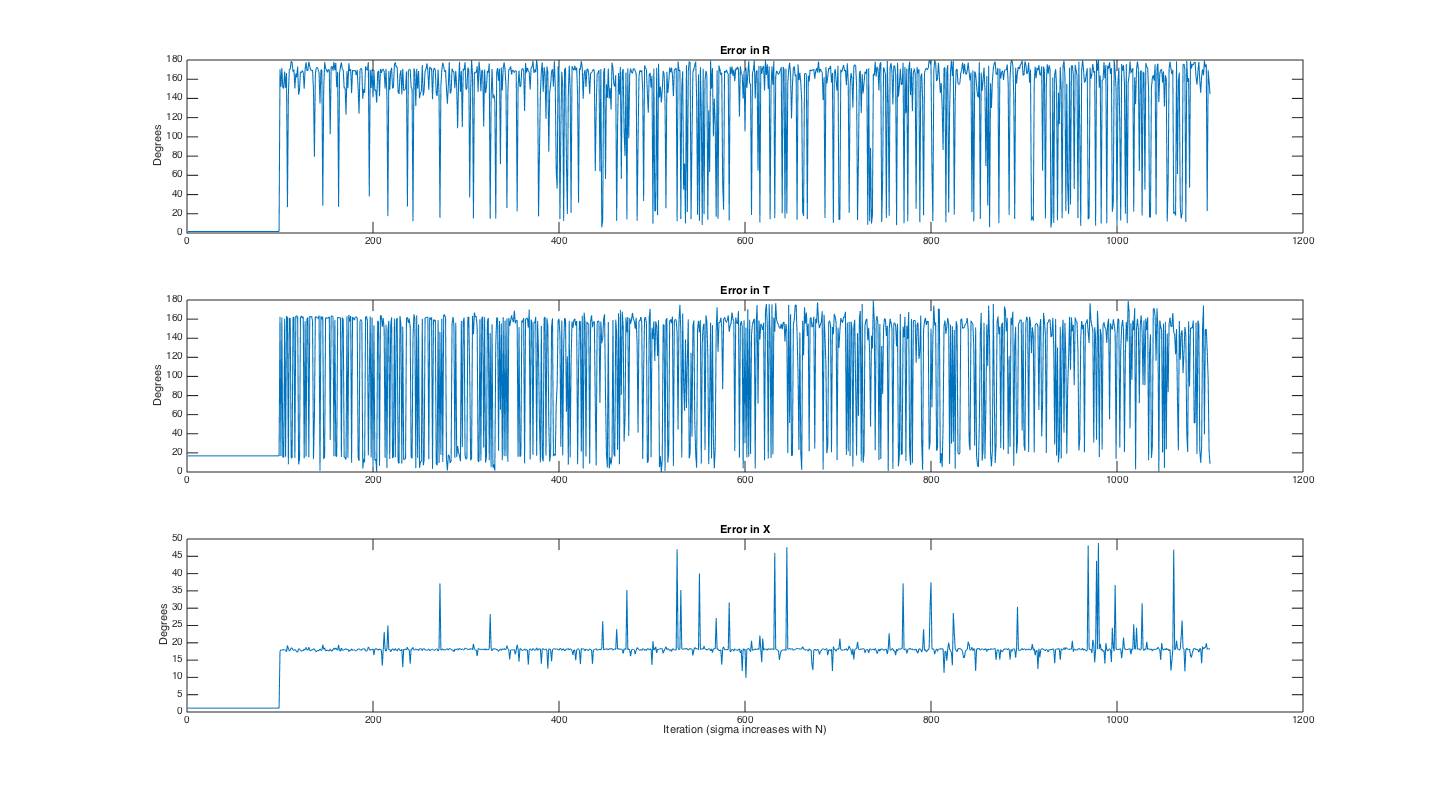
\includegraphics[scale=0.3]{hw5q3.png}

\end{enumerate}
\end{document}
